% chap2.tex


\chapter{Direct Volume rendering using raycasting}\label{chap:errors}

The term volume rendering is used to describe techniques which allow the visualization of three-dimensional data. It is a technique for visualizing sampled functions of three spatial dimensions by computing 2-D projections of a colored semi-transparent volume. In scientific visualization and computer graphics, volume rendering is a set of techniques used to display a 2D projection of a 3D discretely sampled data set, typically a 3D scalar field.

A typical 3D data set is a group of 2D slice images acquired by a CT, MRI, or MicroCT scanner. Usually these are acquired in a regular pattern and usually have a regular number of image pixels in a regular pattern. This is an example of a regular volumetric grid, with each volume element, or voxel represented by a single value that is obtained by sampling the immediate area surrounding the voxel.

\section{Introduction}

Volume rendering involves the following steps: the forming of an RGBA volume from the data, reconstruction of a continuous function from this discrete data set, and projecting it onto the 2D viewing plane (the output image) from the desired point of view. An RGBA volume is a 3D four-vector data set, where the first three components are the familiar R, G, and B color components and the last component, A, represents opacity. An opacity value of 0 means totally transparent and a value of 1 means totally opaque. Behind the RGBA volume an opaque background is placed.

The mapping of the data to opacity values acts as a classification of the data one is interested in. Isosurfaces can be shown by mapping the corresponding data values to almost opaque values and the rest to transparent values. The appearance of surfaces can be improved by using shading techniques to form the RGB mapping. However, opacity can be used to see the interior of the data volume too. These interiors appear as clouds with varying density and color. A big advantage of volume rendering is that this interior information is not thrown away, so that it enables one to look at the 3D data set as a whole. 

\section{Definitions}

\subsection{Voxel}
A voxel represents a single sample, or data point, on a regularly spaced, three-dimensional grid.  It is the basic element of the volume. This data point can consist of a single piece of data, such as an opacity, or multiple pieces of data, such as a color in addition to opacity. A voxel represents only a single point on this grid, not a volume; the space between each voxel is not represented in a voxel-based dataset.

\subsection{Direct Volume rendering}
A direct volume rendering is that visualizations can be created without creating intermediate geometric structure, such
as polygons comprising an isosurface, but simply by a “direct” mapping from volume data points to composited image elements.
Together with traditional computer graphics elements such as camera, lighting, and shading, the central ingredient in that direct map-
ping is the assignment of optical properties (opacity, color, etc.) to the values comprising the volume dataset [1].

[1] Transfer Functions in Direct Volume Rendering: Design, Interface, Interaction Gordon Kindlmann Scientific Computing and Imaging Institute School of Computing University of Utah, SIGGRAPH 2002 notes. 

\subsection{Ray Casting}
Ray casting is a method in which for every pixel in the image, a ray is cast through the volume. The ray intersects a line of voxels.
While passing, the color of the pixel is accumulated according the voxels color and transperacy.

Complexity = O(Depth * ImageSize)

\subsection{Transfer functions}
Transfer function make volume data visible by mapping data values to optical properties, usually done by mapping data values to color and opacity.[2]

[2] Barthold Lichtenbelt, Randy Crane, and Shaz Naqvi. Introduction to Volume Rendering, chapter 4. Prentice-Hall, New
Jersey, 1998.

\section{Volume Ray Casting}

Raycasting is a technique to visualize volume data at interactive frame rates. For every pixel of the image plane a ray is traced through the scene starting from the viewer. The ray equation is given by a starting point and a direction. If the ray hits the volume the color of the pixel is calculated by sampling the data values of the ray at a finite number of positions in the volume. On each sample the transfer function is applied and composited with accumulated values of the ray.

\begin{figure}
\centering
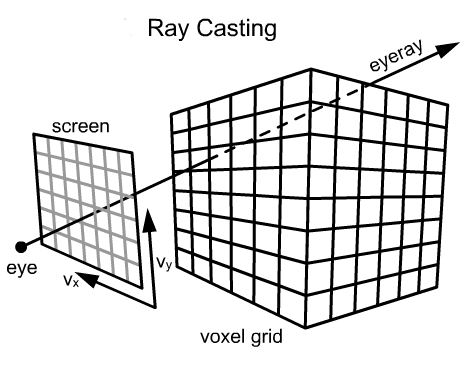
\includegraphics[width=220pt]{Images/ray_cast1.jpg}
\caption{\label{fig:ray_cast1.jpg} Direct Volume rendering using Raycasting.}
\end{figure}

\subsection{Basic Algorithm}

In its basic form, the volume ray casting algorithm comprises of a ray of being cast through the volume, for each pixel of the final image. Generally, the volume is enclosed within a bounding primitive, a simple geometric object — usually a cuboid — that is used to intersect the ray of sight and the volume. Along the part of the ray of sight that lies within the volume, equidistant sampling points or samples are selected. In general, the volume is not aligned with the ray of sight, and sampling points will usually be located in between voxels. Because of that, it is necessary to interpolate the values of the samples from its surrounding voxels, this is called sampling. After all sampling points have been fetched, they are composited along the ray of sight, resulting in the final colour value for the pixel that is currently being processed, this is called compositing, explained in detail at later section.

Raycasting is performed on the GPU. We use two float-textures, where the color value encodes the entry and respectively the exit points. For that we need to pass Entry and Exit params to the relevant fragment program.  To generate these textures we render a cube with an edge length of 1 (from (0,0,0) to (1,1,1)) and set the vertex color to the coordinates. OpenGL will interpolate the color values between the vertices automatically. For the entry points texture we enable back face culling and respectively front face culling for the exit points texture.


Image Entry and Exit Params.

Pseudocode: \\

    Lookup volume entry position  \\
    Lookup volume exit position  \\
    Compute ray of sight direction  \\
    While in volume  \\
        Lookup data value at ray position  \\
        Apply transfer function to data value \\ 
        Accumulate color and opacity  \\
        Advance along ray  \\
	

\subsection{Sampling} 

Along the part of the ray of sight that lies within the volume, equidistant sampling points or samples are selected. In general, the volume is not aligned with the ray of sight, and sampling points will usually be located in between voxels. Because of that, it is necessary to interpolate the values of the samples from its surrounding voxels. (commonly using trilinear interpolation).

\begin{figure}
\centering
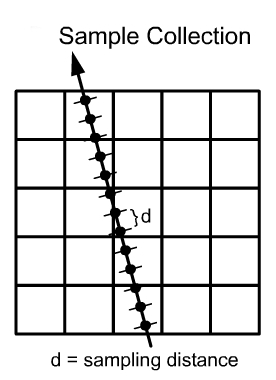
\includegraphics[width=220pt]{Images/sampling1.jpg}
\caption{\label{fig:ray_cast1.jpg} Direct Volume rendering using Raycasting.}
\end{figure}

\subsection{Compositing }

The discrete version of the volume rendering equation replaces the continuous integral with a Riemann sum. 

Discrete Volume Rendering Equations:


$ C \; = \; \sum\limits_{i-1}^{n} \; C_i \; \prod\limits_{j=1}^{i-1} \; ( 1 \; - \; A_j) \; \; $    ...... (2.1)

         
$ A \; = 1 \; - \; \prod\limits_{j=1}^{n} \; ( 1 \; - \; A_j) \; \; $   ...... (2.2) 

Here, Opacity $A_i$ approximates the absorption and opacity-weighted color $C_i$ approximates the emission and the absorption along the ray segment between samples i and i+1. 

This formula is efficiently evaluated by sorting the samples along the viewing ray and computing the accumulated color C and opacity A iteratively. The colour of each sample is determined by classification and shading, and when the transparency is determined by classification, the next step is to evaluate the volume rendering equation. This evaluation is performed by a process called compositing. Two techniques for compositing ray shot into the volume to generate final pixel are front-to-back and back-to-front compositing.


\subsubsection{Back-to-front Compositiong Equations}

In this technique, samples are sorted in back-to-front order, and the accumulated color and opacity are computed iteratively. A single step of the compositing process is known as the Over Operator.  

$  \hat{C}_i \; = \; C_i \; + \; (1 \; - \; A_i ) \; \hat{C}_{i+1}  $   ...... (2.2)

$  \hat{A}_i \; = \; A_i \; + \; (1 \; - \; A_i ) \; \hat{A}_{i+1}  $   ...... (2.3)

where, ${C}_i$ and ${A}_i$ are color and opacity obtained from fragment shading stage for the ray i, along the viewing ray, and $\hat{C}_i$ is the accumulated color from the back of the volume.

\subsubsection{Front-to-Back Compositiong Equations}
In this technique, samples are sorted in front-to-Back order. Front to back compositing is equivalent to back to front, but it has an added advantage. Since the composition is done towards the back and the current transparency is known at all times, the compositing can be stopped early when the translucency is full(nothing behind that point is going to affect the final image). This is one of the more powerful optimizations that can be done for several rendering techniques.

The front to back equation is:

$ \hat{C}_i \; = \; (1 \; - \; \hat{A}_{i-1} \; ) \; C_i \; + \; \hat{C}_{i-1}  $ ...... (2.4)

$ \hat{A}_i \; = \; (1 \; - \; \hat{A}_{i-1} \; ) \; A_i \; + \; \hat{A}_{i-1}  $  ...... (2.5)

where $\hat{C}_i and \hat{A}_i$ are the accumulated color and opacity from the front of the volume. 

